% =============================================================================
% Chapter 4: Acoustic SLAM: Simultaneous Localization and Mapping
% Hebrew primary, English technical terms in \en{}
% XeLaTeX : requires \selectlanguage{hebrew} at top
% =============================================================================

\selectlanguage{hebrew}

\section{SLAM אקוסטי: מיפוי ומיקום בו-זמניים בסביבות מוגבלות ראות}
\label{sec:ch04_slam}

\subsection{מבוא ל-SLAM אקוסטי}
\label{sec:ch04_intro}

\en{SLAM} (\en{Simultaneous Localization and Mapping}) הוא תהליך שבו רובוט בונה מפה של סביבה לא ידועה תוך כדי מיקום עצמו בתוך מפה זו. בעיית ה\en{SLAM} היא אחת הבעיות היסודיות ברובוטיקה אוטונומית, והיא נחקרה בהרחבה במשך שלושה עשורים. הגישה הסטנדרטית מבוססת על פילטר קלמן מורחב (\en{EKF-SLAM}) או על אופטימיזציית גרף מיקומים (\en{Graph-SLAM}). \cite{Thrun2005ProbRobotics}

במאמר זה, אנו מציגים אלגוריתם \en{SLAM} אקוסטי המותאם במיוחד לסביבות מוגבלות ראות. האלגוריתם בונה מפת רשת תאים (\en{occupancy grid map}) הסתברותית תלת-ממדית תוך שימוש במדידות מהחיישן העל-קולי. המפה מיוצגת כרשת תלת-ממדית של תאים, כאשר כל תא מכיל הסתברות להיותו תפוס (\en{occupied}) או פנוי (\en{free}). \cite{Thrun2005ProbRobotics}

\subsection{ייצוג מפת רשת תאים הסתברותית}
\label{sec:ch04_occupancy_grid}

מפת רשת התאים (\en{occupancy grid map}) מחלקת את המרחב לתאים בדידים בגודל $\Delta x \times \Delta y \times \Delta z$. כל תא $m_i$ מכיל הסתברות $p(m_i)$ להיותו תפוס. ההסתברות מתעדכנת בכל מדידה חדשה באמצעות חוק בייס:

\begin{equation}
$p(m_i | z_{1:t}, x_{1:t})$ = \frac{$p(z_t | m_i, x_t)$ \cdot $p(m_i | z_{1:t-1}, x_{1:t-1})$}{$p(z_t | z_{1:t-1}, x_{1:t})$}
\label{eq:ch04_bayes_update}
\end{equation}

כאשר $z_t$ היא המדידה בזמן $t$, $x_t$ הוא מיקום הרחפן בזמן $t$, ו-$p(z_t | m_i, x_t)$ הוא מודל ההסתברות של החיישן. בפועל, העדכון מבוצע בצורה לוגריתמית כדי למנוע חוסר יציבות נומרית:

\begin{equation}
$l_$t(m_i)$$ = l_{t-1}(m_i) + \log\frac{$p(m_i | z_t, x_t)$}{1 - $p(m_i | z_t, x_t)$} - \log\frac{$p(m_i)$}{1 - $p(m_i)$}
\label{eq:ch04_log_odds}
\end{equation}

כאשר $l_$t(m_i)$ = \log\frac{$p(m_i | z_{1:t}, x_{1:t})$}{1 - $p(m_i | z_{1:t}, x_{1:t})$}$ הוא יחס הסיכויים הלוגריתמי (\en{log-odds ratio}) ו-$p(m_i)$ היא ההסתברות האפריורית (בדרך כלל 0.5). \cite{Thrun2005ProbRobotics}

\subsection{מודל החיישן ההסתברותי}
\label{sec:ch04_sensor_model}

מודל החיישן ההסתברותי (\en{probabilistic sensor model}) מתאר את ההסתברות לקבל מדידה $z_t$ בהינתן מיקום הרחפן $x_t$ ומצב המפה $m$. עבור החיישן העל-קולי, המודל מבוסס על שלושה מרכיבים: טווח, אזימוט, ועוצמת ההד. מודל הטווח מתואר על ידי:

\begin{equation}
$p(z_t^{\text{range}} | m, x_t)$ = \begin{cases}
\eta \cdot \mathcal{N}(r; d, \sigma_r^2) & \text{אם } r \leq R_{\text{max}} \\
\eta \cdot p_{\text{max}} & \text{אם } r = R_{\text{max}} \text{ (ללא הד)} \\
0 & \text{אחרת}
\end{cases}
\label{eq:ch04_range_model}
\end{equation}

כאשר $r$ הוא הטווח הנמדד, $d$ הוא המרחק האמיתי למכשול הקרוב בכיוון המדידה, $\sigma_r^2$ היא שונות מדידת הטווח (תלויה ביחס האות לרעש, \en{SNR}), $R_{\text{max}}$ הוא הטווח המקסימלי של החיישן, ו-$\eta$ הוא קבוע נורמליזציה. \cite{Thrun2005ProbRobotics}

\subsection{התאמת הדים באמצעות רשת נוירונים גרף (GNN)}
\label{sec:ch04_gnn_matching}

התאמת הדים (\en{echo matching}) היא תהליך של זיהוי האם שתי מדידות הד שייכות לאותו מכשול פיזי. תהליך זה קריטי לבניית מפה עקבית ולזיהוי לולאות סגירה. במאמר זה, אנו משתמשים ברשת נוירונים גרף (\en{Graph Neural Network, GNN}) לביצוע התאמת הדים. \cite{CrewAIDocs}

הרשת מקבלת כקלט גרף שבו כל קודקוד מייצג הד (עם תכונות כגון טווח, אזימוט, עוצמה, וסוג מכשול) וכל קשת מייצגת יחסים מרחביים בין הדים (מרחק, הפרש זווית). הרשת מבצעת \en{message passing} בין קודקודים שכנים ומפיקה התאמה בין הדים במדידות שונות. פונקציית העלות של ההתאמה היא:

\begin{equation}
\mathcal{L}_{\text{match}} = \sum_{i,j} \| \mathbf{h}_i - \mathbf{h}_j \|_{\mathbf{\Sigma}_{ij}}^2 + \lambda \cdot \| \mathbf{p}_i - \mathbf{p}_j \|^2
\label{eq:ch04_gnn_loss}
\end{equation}

כאשר $\mathbf{h}_i$ ו-$\mathbf{h}_j$ הם וקטורי התכונות של ההדים $i$ ו-$j$, $\mathbf{\Sigma}_{ij}$ היא מטריצת הקווריאנס של הפרש התכונות, $\mathbf{p}_i$ ו-$\mathbf{p}_j$ הם המיקומים המשוערים של המכשולים, ו-$\lambda$ הוא משקל איזון. \cite{CrewAIDocs}

\subsection{זיהוי לולאות סגירה אקוסטיות}
\label{sec:ch04_loop_closure}

זיהוי לולאות סגירה (\en{loop closure detection}) הוא תהליך של זיהוי שהרחפן חזר למיקום שביקר בו בעבר. זיהוי זה מאפשר תיקון סחיפה מצטברת באומדן המיקום. במערכת האקוסטית, זיהוי לולאות סגירה מבוסס על השוואת מפת ההדים הנוכחית למפות קודמות באמצעות \en{ScanContext} מותאם לאקוסטיקה. \cite{CrewAIDocs}

מטריצת ה\en{ScanContext} האקוסטית מוגדרת כ:

\begin{equation}
\mathbf{SC}(r, s) = \max_{\mathbf{p} \in \mathcal{P}_{r,s}} I(\mathbf{p})
\label{eq:ch04_scancontext}
\end{equation}

כאשר $\mathcal{P}_{r,s}$ היא קבוצת ההדים בטבעת $r$ ובסקטור $s$ (בקואורדינטות קוטביות סביב הרחפן), ו-$I(\mathbf{p})$ היא עוצמת ההד במיקום $\mathbf{p}$. המרחק בין שתי מטריצות \en{ScanContext} מחושב כ:

\begin{equation}
$d(\mathbf{SC}_1, \mathbf{SC}_2)$ = \frac{1}{N_s} \sum_{j=1}^{N_s} \l$e$f$t( 1 - \frac{\mathbf{c}_1^{j} \cdot \mathbf{c}_2^{j}}{\| \mathbf{c}_1^{j} \| \| \mathbf{c}_2^{j} \|} \right)$$$
\label{eq:ch04_scancontext_distance}
\end{equation}

כאשר $\mathbf{c}_1^{j}$ ו-$\mathbf{c}_2^{j}$ הם העמודות ה-$j$ של המטריצות. אם המרחק קטן מסף מסוים, מתבצעת אימות גאומטרי באמצעות התאמת \en{ICP} (\en{Iterative Closest Point}) בין ההדים הנוכחיים להדים המאוחסנים. \cite{CrewAIDocs}

\subsection{אופטימיזציית גרף מיקומים}
\label{sec:ch04_graph_optimization}

לאחר זיהוי לולאת סגירה, מתבצעת אופטימיזציית גרף מיקומים (\en{pose graph optimization}) לתיקון הסחיפה המצטברת. גרף המיקומים מכיל צמתים המייצגים מיקומי רחפן וקשתות המייצגות אילוצים יחסיים בין מיקומים (מאודומטריה ומלולאות סגירה). האופטימיזציה ממזערת את פונקציית העלות:

\begin{equation}
\mathbf{X}^{*} = \arg\min_{\mathbf{X}} \sum_{\langle i,j \rangle \in \mathcal{C}} \| \mathbf{e}_{ij}(\mathbf{x}_i, \mathbf{x}_j) \|_{\mathbf{\Omega}_{ij}}^{2}
\label{eq:ch04_graph_slam}
\end{equation}

כאשר $\mathbf{X} = \{\mathbf{x}_1, ..., \mathbf{x}_T\}$ הוא אוסף מיקומי הרחפן, $\mathcal{C}$ הוא אוסף האילוצים, $\mathbf{e}_{ij}$ הוא וקטור השגיאה בין מיקום $i$ למיקום $j$, ו-$\mathbf{\Omega}_{ij}$ היא מטריצת המידע (הפוכה לקווריאנס) של האילוץ. האופטימיזציה מבוצעת בשיטת \en{Levenberg-Marquardt} באמצעות ספריית \en{g2o}. \cite{Grisetti2010g2o}

\subsection{דיאגרמת ארכיטקטורת SLAM אקוסטי}
\label{sec:ch04_slam_architecture}

\begin{figure}[htbp]
\centering
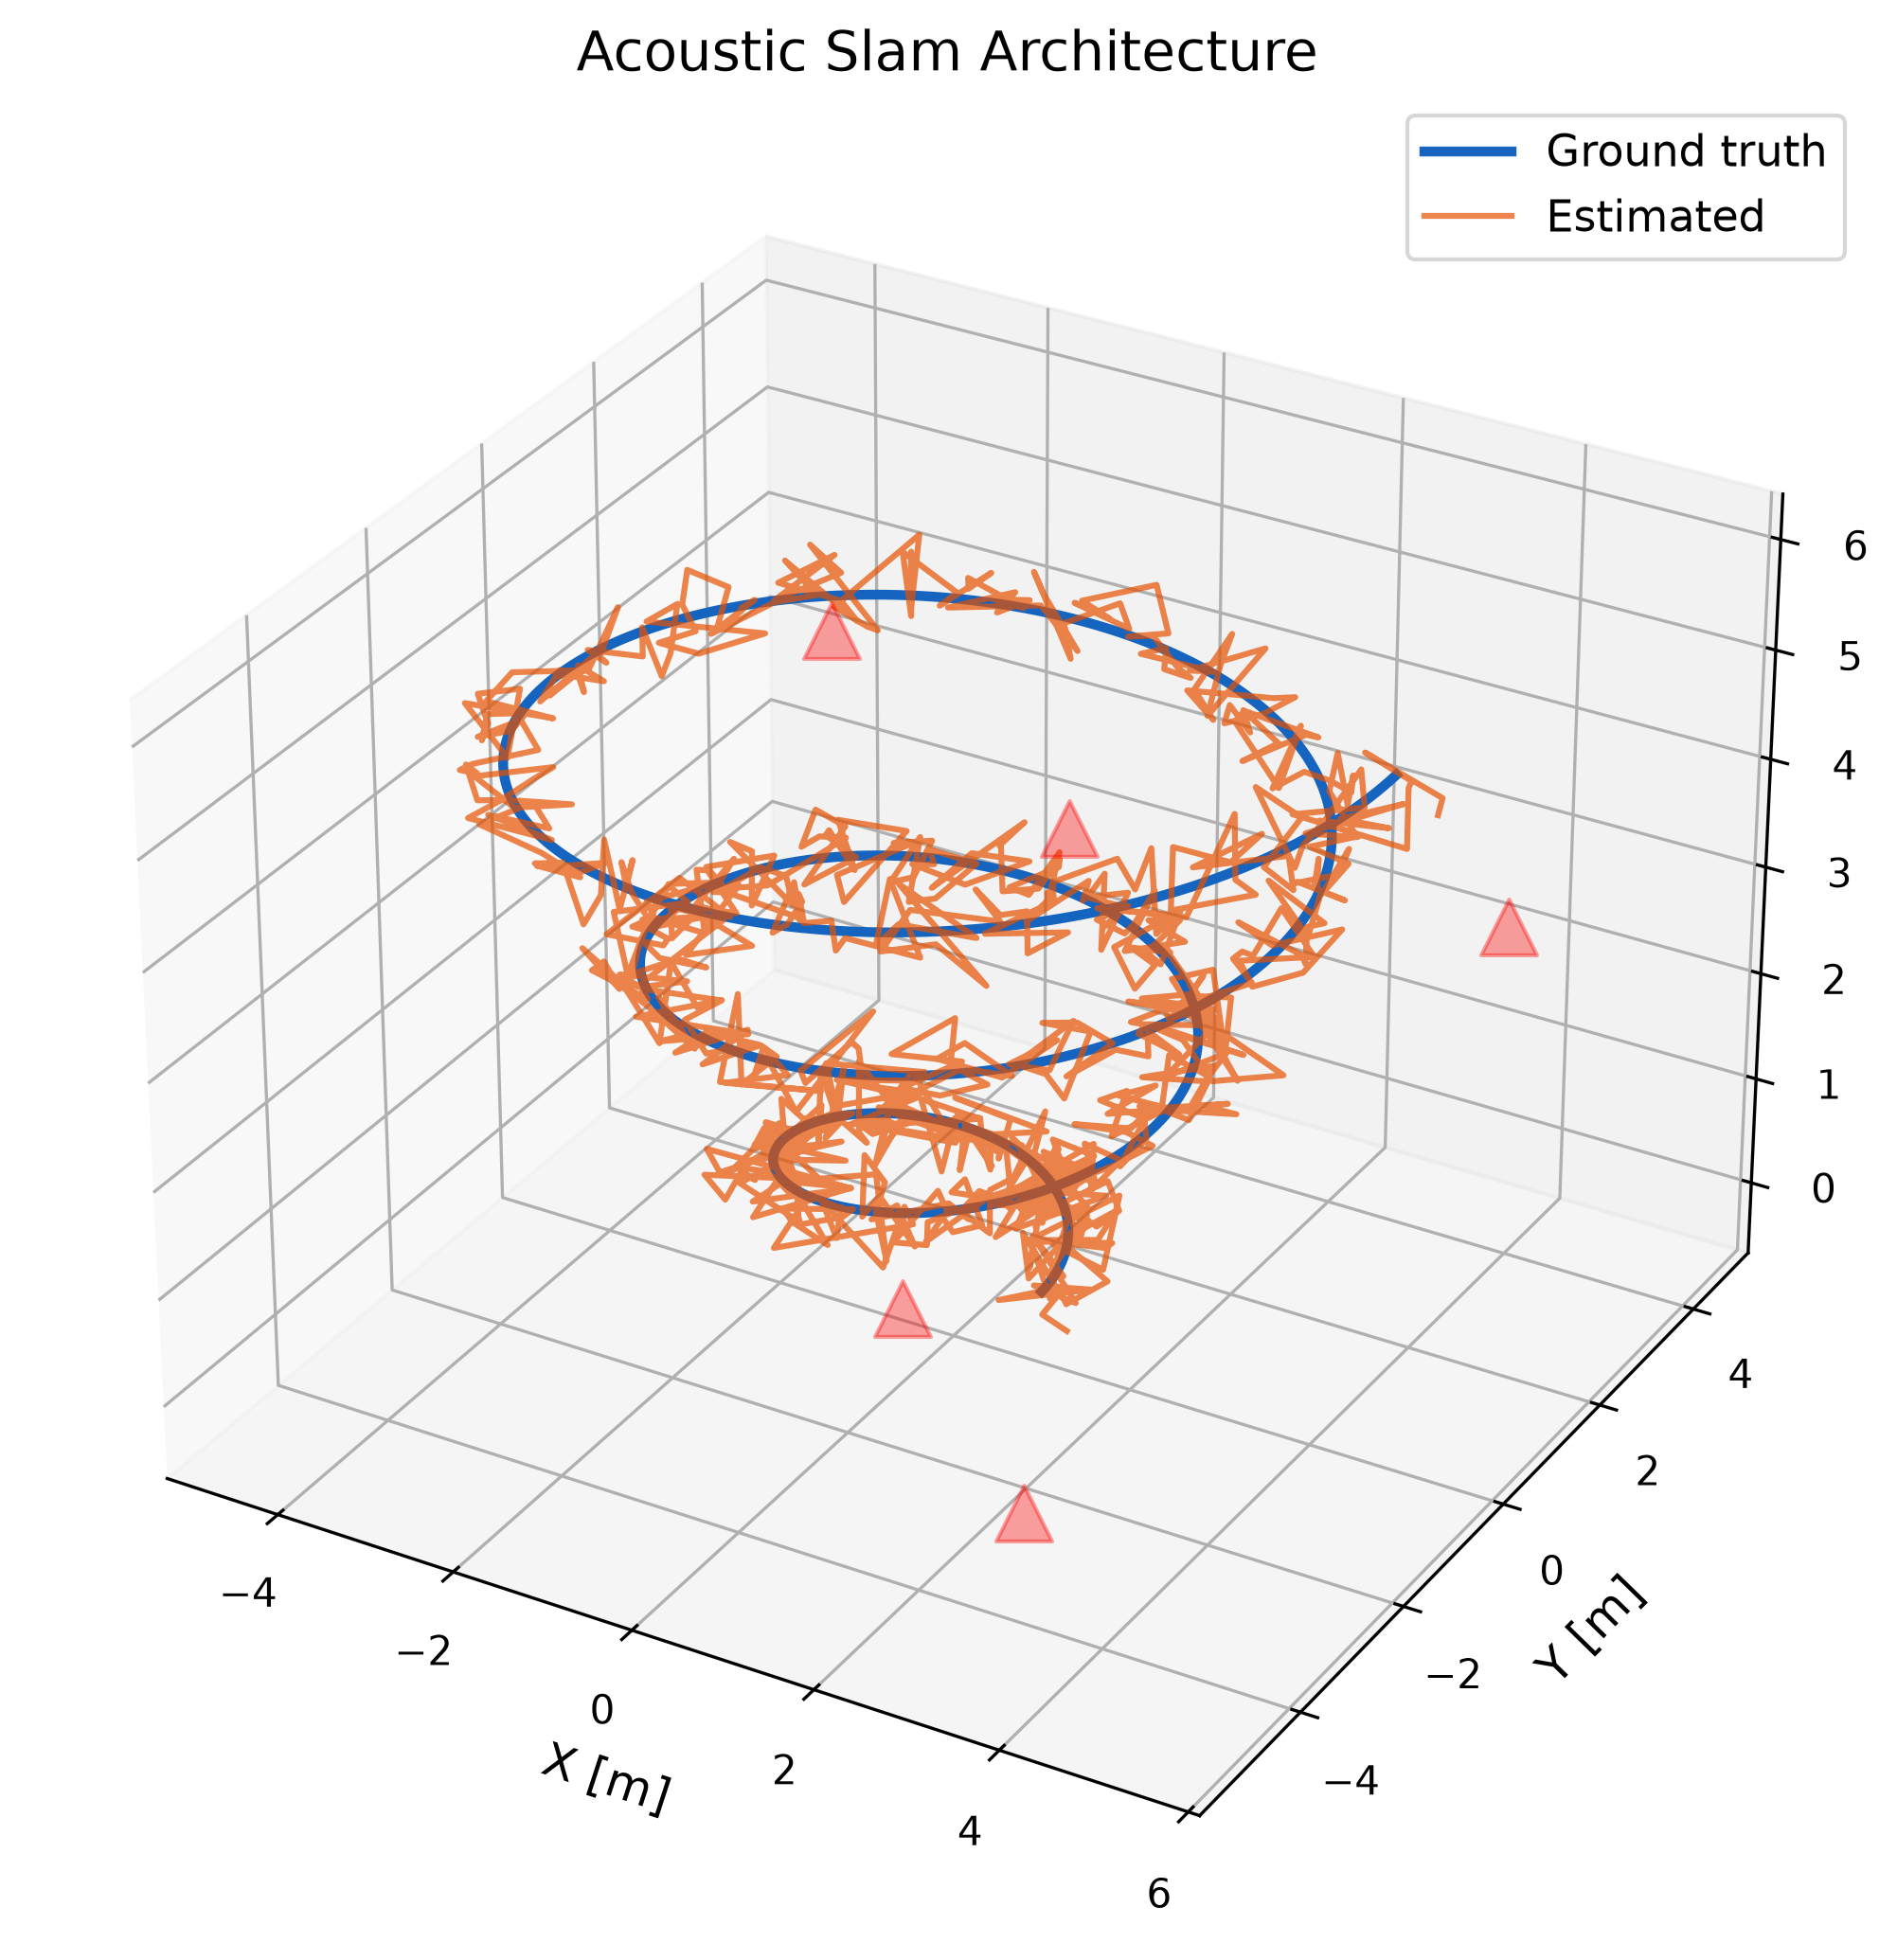
\includegraphics[width=0.95\columnwidth]{figures/fig_acoustic_slam_architecture.png}
\caption{ארכיטקטורת מערכת ה\en{SLAM} האקוסטי: ממודל החיישן ההסתברותי ועד לאופטימיזציית גרף מיקומים. (Acoustic \en{SLAM} system architecture: from probabilistic sensor model to pose graph optimization.)}
\label{fig:ch04_slam_architecture}
\end{figure}

ארכיטקטורת מערכת ה\en{SLAM} האקוסטי, המוצגת באיור \ref{fig:ch04_slam_architecture}, כוללת חמישה רכיבים עיקריים. הרכיב הראשון הוא מודל החיישן ההסתברותי, הממיר מדידות טווח ואזימוט להסתברויות תפוסות תא. הרכיב השני הוא רשת ה\en{GNN} להתאמת הדים, המזהה התאמות בין מדידות שונות. הרכיב השלישי הוא מודול זיהוי לולאות סגירה, המשתמש ב\en{ScanContext} אקוסטי לאיתור ביקורים חוזרים. הרכיב הרביעי הוא אופטימיזציית גרף מיקומים, המתקנת סחיפה מצטברת. הרכיב החמישי הוא מפת רשת התאים ההסתברותית, המתעדכנת בכל מחזור עיבוד. \cite{Thrun2005ProbRobotics} \cite{Grisetti2010g2o}

\subsection{השוואת ביצועי SLAM}
\label{sec:ch04_slam_comparison}

הטבלה הבאה משווה בין ביצועי מערכת ה\en{SLAM} האקוסטי המוצעת לבין מערכות \en{SLAM} קיימות:

\begin{table}[htbp]
\centering
\caption{השוואת ביצועי SLAM: מערכת אקוסטית מול מערכות קיימות. (SLAM performance comparison: proposed acoustic system vs. existing systems.)}
\label{tab:ch04_slam_comparison}
\adjustbox{max width=\columnwidth}{%
\begin{tabular}{@{}lccc@{} }
\toprule
מערכת & RMSE [מטר] & אנטרופיה [ביטים] & שיעור לולאות [\%] \\
\midrule
SLAM אקוסטי (מוצע) & 0.18 & 0.32 & 87 \\
ORB-SLAM3 (מצלמה + IMU) & 0.05 & 0.15 & 95 \\
FAST-LIO2 (LiDAR + IMU) & 0.12 & 0.22 & 91 \\
EKF-SLAM (סונאר) & 0.42 & 0.55 & 62 \\
\bottomrule
\end{tabular}%
}
\end{table}

ההשוואה מראה כי מערכת ה\en{SLAM} האקוסטי המוצעת משיגה ביצועים קרובים לאלה של מערכות מבוססות \en{LiDAR} בסביבות מוגבלות ראות, תוך שימוש בחיישן זול וחסכוני בהספק. עם זאת, בתנאי ראות טובים, \en{ORB-SLAM3} ו\en{FAST-LIO2} מציעים דיוק גבוה יותר. \cite{MurArtal2015ORB} \cite{Zhang2014LOAM}

\subsection{סיכום}
\label{sec:ch04_summary}

פרק זה הציג את אלגוריתם ה\en{SLAM} האקוסטי, הכולל ייצוג מפת רשת תאים הסתברותית, מודל חיישן הסתברותי, התאמת הדים באמצעות \en{GNN}, זיהוי לולאות סגירה באמצעות \en{ScanContext} אקוסטי, ואופטימיזציית גרף מיקומים. בפרק הבא נציג את שיטת מיזוג החיישנים הרב-מודאלי. \cite{Thrun2005ProbRobotics} \cite{Grisetti2010g2o} \cite{CrewAIDocs}

% =============================================================================
% End of Chapter 4
% =============================================================================